%% template.tex
%% from
%% bare_conf.tex
%% V1.4b
%% 2015/08/26
%% by Michael Shell
%% See:
%% http://www.michaelshell.org/
%% for current contact information.
%%
%% This is a skeleton file demonstrating the use of IEEEtran.cls
%% (requires IEEEtran.cls version 1.8b or later) with an IEEE
%% conference paper.
%%
%% Support sites:
%% http://www.michaelshell.org/tex/ieeetran/
%% http://www.ctan.org/pkg/ieeetran
%% and
%% http://www.ieee.org/

%%*************************************************************************
%% Legal Notice:
%% This code is offered as-is without any warranty either expressed or
%% implied; without even the implied warranty of MERCHANTABILITY or
%% FITNESS FOR A PARTICULAR PURPOSE!
%% User assumes all risk.
%% In no event shall the IEEE or any contributor to this code be liable for
%% any damages or losses, including, but not limited to, incidental,
%% consequential, or any other damages, resulting from the use or misuse
%% of any information contained here.
%%
%% All comments are the opinions of their respective authors and are not
%% necessarily endorsed by the IEEE.
%%
%% This work is distributed under the LaTeX Project Public License (LPPL)
%% ( http://www.latex-project.org/ ) version 1.3, and may be freely used,
%% distributed and modified. A copy of the LPPL, version 1.3, is included
%% in the base LaTeX documentation of all distributions of LaTeX released
%% 2003/12/01 or later.
%% Retain all contribution notices and credits.
%% ** Modified files should be clearly indicated as such, including  **
%% ** renaming them and changing author support contact information. **
%%*************************************************************************


% *** Authors should verify (and, if needed, correct) their LaTeX system  ***
% *** with the testflow diagnostic prior to trusting their LaTeX platform ***
% *** with production work. The IEEE's font choices and paper sizes can   ***
% *** trigger bugs that do not appear when using other class files.       ***                          ***
% The testflow support page is at:
% http://www.michaelshell.org/tex/testflow/

\documentclass[conference,final,]{IEEEtran}
% Some Computer Society conferences also require the compsoc mode option,
% but others use the standard conference format.
%
% If IEEEtran.cls has not been installed into the LaTeX system files,
% manually specify the path to it like:
% \documentclass[conference]{../sty/IEEEtran}





% Some very useful LaTeX packages include:
% (uncomment the ones you want to load)


% *** MISC UTILITY PACKAGES ***
%
%\usepackage{ifpdf}
% Heiko Oberdiek's ifpdf.sty is very useful if you need conditional
% compilation based on whether the output is pdf or dvi.
% usage:
% \ifpdf
%   % pdf code
% \else
%   % dvi code
% \fi
% The latest version of ifpdf.sty can be obtained from:
% http://www.ctan.org/pkg/ifpdf
% Also, note that IEEEtran.cls V1.7 and later provides a builtin
% \ifCLASSINFOpdf conditional that works the same way.
% When switching from latex to pdflatex and vice-versa, the compiler may
% have to be run twice to clear warning/error messages.






% *** CITATION PACKAGES ***
%
%\usepackage{cite}
% cite.sty was written by Donald Arseneau
% V1.6 and later of IEEEtran pre-defines the format of the cite.sty package
% \cite{} output to follow that of the IEEE. Loading the cite package will
% result in citation numbers being automatically sorted and properly
% "compressed/ranged". e.g., [1], [9], [2], [7], [5], [6] without using
% cite.sty will become [1], [2], [5]--[7], [9] using cite.sty. cite.sty's
% \cite will automatically add leading space, if needed. Use cite.sty's
% noadjust option (cite.sty V3.8 and later) if you want to turn this off
% such as if a citation ever needs to be enclosed in parenthesis.
% cite.sty is already installed on most LaTeX systems. Be sure and use
% version 5.0 (2009-03-20) and later if using hyperref.sty.
% The latest version can be obtained at:
% http://www.ctan.org/pkg/cite
% The documentation is contained in the cite.sty file itself.






% *** GRAPHICS RELATED PACKAGES ***
%
\ifCLASSINFOpdf
  % \usepackage[pdftex]{graphicx}
  % declare the path(s) where your graphic files are
  % \graphicspath{{../pdf/}{../jpeg/}}
  % and their extensions so you won't have to specify these with
  % every instance of \includegraphics
  % \DeclareGraphicsExtensions{.pdf,.jpeg,.png}
\else
  % or other class option (dvipsone, dvipdf, if not using dvips). graphicx
  % will default to the driver specified in the system graphics.cfg if no
  % driver is specified.
  % \usepackage[dvips]{graphicx}
  % declare the path(s) where your graphic files are
  % \graphicspath{{../eps/}}
  % and their extensions so you won't have to specify these with
  % every instance of \includegraphics
  % \DeclareGraphicsExtensions{.eps}
\fi
% graphicx was written by David Carlisle and Sebastian Rahtz. It is
% required if you want graphics, photos, etc. graphicx.sty is already
% installed on most LaTeX systems. The latest version and documentation
% can be obtained at:
% http://www.ctan.org/pkg/graphicx
% Another good source of documentation is "Using Imported Graphics in
% LaTeX2e" by Keith Reckdahl which can be found at:
% http://www.ctan.org/pkg/epslatex
%
% latex, and pdflatex in dvi mode, support graphics in encapsulated
% postscript (.eps) format. pdflatex in pdf mode supports graphics
% in .pdf, .jpeg, .png and .mps (metapost) formats. Users should ensure
% that all non-photo figures use a vector format (.eps, .pdf, .mps) and
% not a bitmapped formats (.jpeg, .png). The IEEE frowns on bitmapped formats
% which can result in "jaggedy"/blurry rendering of lines and letters as
% well as large increases in file sizes.
%
% You can find documentation about the pdfTeX application at:
% http://www.tug.org/applications/pdftex





% *** MATH PACKAGES ***
%
%\usepackage{amsmath}
% A popular package from the American Mathematical Society that provides
% many useful and powerful commands for dealing with mathematics.
%
% Note that the amsmath package sets \interdisplaylinepenalty to 10000
% thus preventing page breaks from occurring within multiline equations. Use:
%\interdisplaylinepenalty=2500
% after loading amsmath to restore such page breaks as IEEEtran.cls normally
% does. amsmath.sty is already installed on most LaTeX systems. The latest
% version and documentation can be obtained at:
% http://www.ctan.org/pkg/amsmath





% *** SPECIALIZED LIST PACKAGES ***
%
%\usepackage{algorithmic}
% algorithmic.sty was written by Peter Williams and Rogerio Brito.
% This package provides an algorithmic environment fo describing algorithms.
% You can use the algorithmic environment in-text or within a figure
% environment to provide for a floating algorithm. Do NOT use the algorithm
% floating environment provided by algorithm.sty (by the same authors) or
% algorithm2e.sty (by Christophe Fiorio) as the IEEE does not use dedicated
% algorithm float types and packages that provide these will not provide
% correct IEEE style captions. The latest version and documentation of
% algorithmic.sty can be obtained at:
% http://www.ctan.org/pkg/algorithms
% Also of interest may be the (relatively newer and more customizable)
% algorithmicx.sty package by Szasz Janos:
% http://www.ctan.org/pkg/algorithmicx




% *** ALIGNMENT PACKAGES ***
%
%\usepackage{array}
% Frank Mittelbach's and David Carlisle's array.sty patches and improves
% the standard LaTeX2e array and tabular environments to provide better
% appearance and additional user controls. As the default LaTeX2e table
% generation code is lacking to the point of almost being broken with
% respect to the quality of the end results, all users are strongly
% advised to use an enhanced (at the very least that provided by array.sty)
% set of table tools. array.sty is already installed on most systems. The
% latest version and documentation can be obtained at:
% http://www.ctan.org/pkg/array


% IEEEtran contains the IEEEeqnarray family of commands that can be used to
% generate multiline equations as well as matrices, tables, etc., of high
% quality.




% *** SUBFIGURE PACKAGES ***
%\ifCLASSOPTIONcompsoc
%  \usepackage[caption=false,font=normalsize,labelfont=sf,textfont=sf]{subfig}
%\else
%  \usepackage[caption=false,font=footnotesize]{subfig}
%\fi
% subfig.sty, written by Steven Douglas Cochran, is the modern replacement
% for subfigure.sty, the latter of which is no longer maintained and is
% incompatible with some LaTeX packages including fixltx2e. However,
% subfig.sty requires and automatically loads Axel Sommerfeldt's caption.sty
% which will override IEEEtran.cls' handling of captions and this will result
% in non-IEEE style figure/table captions. To prevent this problem, be sure
% and invoke subfig.sty's "caption=false" package option (available since
% subfig.sty version 1.3, 2005/06/28) as this is will preserve IEEEtran.cls
% handling of captions.
% Note that the Computer Society format requires a larger sans serif font
% than the serif footnote size font used in traditional IEEE formatting
% and thus the need to invoke different subfig.sty package options depending
% on whether compsoc mode has been enabled.
%
% The latest version and documentation of subfig.sty can be obtained at:
% http://www.ctan.org/pkg/subfig




% *** FLOAT PACKAGES ***
%

%\usepackage{fixltx2e}
% fixltx2e, the successor to the earlier fix2col.sty, was written by
% Frank Mittelbach and David Carlisle. This package corrects a few problems
% in the LaTeX2e kernel, the most notable of which is that in current
% LaTeX2e releases, the ordering of single and double column floats is not
% guaranteed to be preserved. Thus, an unpatched LaTeX2e can allow a
% single column figure to be placed prior to an earlier double column
% figure.
% Be aware that LaTeX2e kernels dated 2015 and later have fixltx2e.sty's
% corrections already built into the system in which case a warning will
% be issued if an attempt is made to load fixltx2e.sty as it is no longer
% needed.
% The latest version and documentation can be found at:
% http://www.ctan.org/pkg/fixltx2e


%\usepackage{stfloats}
% stfloats.sty was written by Sigitas Tolusis. This package gives LaTeX2e
% the ability to do double column floats at the bottom of the page as well
% as the top. (e.g., "\begin{figure*}[!b]" is not normally possible in
% LaTeX2e). It also provides a command:
%\fnbelowfloat
% to enable the placement of footnotes below bottom floats (the standard
% LaTeX2e kernel puts them above bottom floats). This is an invasive package
% which rewrites many portions of the LaTeX2e float routines. It may not work
% with other packages that modify the LaTeX2e float routines. The latest
% version and documentation can be obtained at:
% http://www.ctan.org/pkg/stfloats
% Do not use the stfloats baselinefloat ability as the IEEE does not allow
% \baselineskip to stretch. Authors submitting work to the IEEE should note
% that the IEEE rarely uses double column equations and that authors should try
% to avoid such use. Do not be tempted to use the cuted.sty or midfloat.sty
% packages (also by Sigitas Tolusis) as the IEEE does not format its papers in
% such ways.
% Do not attempt to use stfloats with fixltx2e as they are incompatible.
% Instead, use Morten Hogholm'a dblfloatfix which combines the features
% of both fixltx2e and stfloats:
%
% \usepackage{dblfloatfix}
% The latest version can be found at:
% http://www.ctan.org/pkg/dblfloatfix




% *** PDF, URL AND HYPERLINK PACKAGES ***
%
%\usepackage{url}
% url.sty was written by Donald Arseneau. It provides better support for
% handling and breaking URLs. url.sty is already installed on most LaTeX
% systems. The latest version and documentation can be obtained at:
% http://www.ctan.org/pkg/url
% Basically, \url{my_url_here}.




% *** Do not adjust lengths that control margins, column widths, etc. ***
% *** Do not use packages that alter fonts (such as pslatex).         ***
% There should be no need to do such things with IEEEtran.cls V1.6 and later.
% (Unless specifically asked to do so by the journal or conference you plan
% to submit to, of course. )



%% BEGIN MY ADDITIONS %%


\usepackage{graphicx}
% We will generate all images so they have a width \maxwidth. This means
% that they will get their normal width if they fit onto the page, but
% are scaled down if they would overflow the margins.
\makeatletter
\def\maxwidth{\ifdim\Gin@nat@width>\linewidth\linewidth
\else\Gin@nat@width\fi}
\makeatother
\let\Oldincludegraphics\includegraphics
\renewcommand{\includegraphics}[1]{\Oldincludegraphics[width=\maxwidth]{#1}}

\usepackage[unicode=true]{hyperref}

\hypersetup{
            pdftitle={Visual Inference Test of the Hexagon Tile Map for Spatial Distributions},
            pdfkeywords={statistics, visual inference, geospatial, population},
            pdfborder={0 0 0},
            breaklinks=true}
\urlstyle{same}  % don't use monospace font for urls

% Pandoc toggle for numbering sections (defaults to be off)
\setcounter{secnumdepth}{0}

% Pandoc syntax highlighting

% Pandoc header

\providecommand{\tightlist}{%
  \setlength{\itemsep}{0pt}\setlength{\parskip}{0pt}}

%% END MY ADDITIONS %%


\hyphenation{op-tical net-works semi-conduc-tor}

\begin{document}
%
% paper title
% Titles are generally capitalized except for words such as a, an, and, as,
% at, but, by, for, in, nor, of, on, or, the, to and up, which are usually
% not capitalized unless they are the first or last word of the title.
% Linebreaks \\ can be used within to get better formatting as desired.
% Do not put math or special symbols in the title.
\title{Visual Inference Test of the Hexagon Tile Map for Spatial Distributions}

% author names and affiliations
% use a multiple column layout for up to three different
% affiliations

\author{

%% ---- classic IEEETrans wide authors' list ----------------
 % -- end affiliation.wide
%% ----------------------------------------------------------



%% ---- classic IEEETrans one column per institution --------
 %% -- end if/affiliation.institution-columnar
%% ----------------------------------------------------------





%% ---- one column per author, classic/default IEEETrans ----
 % -- beg affiliation.author-columnar
  %% -- beg for/affiliation.institution.author
\IEEEauthorblockN{
Stephanie Kobakian
}
\IEEEauthorblockA{Queensland University of Technology\\
Science and Engineering Faculty\\
Brisbane, Australia
\\stephanie.kobakian@qut.edu.au
}
 %% -- end for/affiliation.institution.author
\and
  %% -- beg for/affiliation.institution.author
\IEEEauthorblockN{
Dianne Cook
}
\IEEEauthorblockA{Monash University\\
Econometrics and Business Statistics Faculty\\
Melbourne, Australia
\\dicook@monash.edu
}
 %% -- end for/affiliation.institution.author
 %% -- end for/affiliation.institution
 %% -- end if/affiliation.institution-columnar
%% ----------------------------------------------------------

}

% conference papers do not typically use \thanks and this command
% is locked out in conference mode. If really needed, such as for
% the acknowledgment of grants, issue a \IEEEoverridecommandlockouts
% after \documentclass

% for over three affiliations, or if they all won't fit within the width
% of the page, use this alternative format:
%
%\author{\IEEEauthorblockN{Michael Shell\IEEEauthorrefmark{1},
%Homer Simpson\IEEEauthorrefmark{2},
%James Kirk\IEEEauthorrefmark{3},
%Montgomery Scott\IEEEauthorrefmark{3} and
%Eldon Tyrell\IEEEauthorrefmark{4}}
%\IEEEauthorblockA{\IEEEauthorrefmark{1}School of Electrical and Computer Engineering\\
%Georgia Institute of Technology,
%Atlanta, Georgia 30332--0250\\ Email: see http://www.michaelshell.org/contact.html}
%\IEEEauthorblockA{\IEEEauthorrefmark{2}Twentieth Century Fox, Springfield, USA\\
%Email: homer@thesimpsons.com}
%\IEEEauthorblockA{\IEEEauthorrefmark{3}Starfleet Academy, San Francisco, California 96678-2391\\
%Telephone: (800) 555--1212, Fax: (888) 555--1212}
%\IEEEauthorblockA{\IEEEauthorrefmark{4}Tyrell Inc., 123 Replicant Street, Los Angeles, California 90210--4321}}




% use for special paper notices
%\IEEEspecialpapernotice{(Invited Paper)}




% make the title area
\maketitle

% As a general rule, do not put math, special symbols or citations
% in the abstract
\begin{abstract}
The abstract goes here. On multiple lines eventually.
\end{abstract}

% keywords
\begin{IEEEkeywords}
statistics; visual inference; geospatial; population
\end{IEEEkeywords}

% use for special paper notices



% make the title area
\maketitle

% no keywords

% For peer review papers, you can put extra information on the cover
% page as needed:
% \ifCLASSOPTIONpeerreview
% \begin{center} \bfseries EDICS Category: 3-BBND \end{center}
% \fi
%
% For peerreview papers, this IEEEtran command inserts a page break and
% creates the second title. It will be ignored for other modes.
\IEEEpeerreviewmaketitle


\hypertarget{introduction}{%
\section{Introduction}\label{introduction}}

Geo-spatial statistics are often presented on the geographic map base.
To present geo-spatial population statistics, information for
individuals within each geographic region are often aggregated. A
choropleth map is the common display to present aggreagated statistics
for geographic units, and they are often used to present statistics
regarding the population. This visualisation method involves drawing the
administrative boundaries and filling them with colour to communicate
the value of the statistic. In Australia, there are many sets of
administrative boundaries that define subdivisions of the population at
various granularities.

When presenting population statistics on a geographic map base, the size
of the regions can allow errornous conclusions to be drawn about the
state of the statistic over the entire population. This occurs as large
regions filled with a consistent colour or pettern can draw the
attention of map readers, and small regions are not paid equal
attention.

\hypertarget{background-and-motivation}{%
\section{Background and Motivation}\label{background-and-motivation}}

\hypertarget{australian-cancer-atlas}{%
\subsection{Australian Cancer Atlas}\label{australian-cancer-atlas}}

\begin{itemize}
\tightlist
\item
  Communicating spatial distributions
\item
  Trend over geographic space
\item
  Trend over communities and populations
\end{itemize}

The Australian Cancer Atlas explores the burden of cancer on Australian
communities. There are many cancer types presented, and they can be
explored on an individual or aggregate level. The Australian communities
examined are Statistical Areas at Level 2 (SA2)(``Australian Statistical
Geography Standard (ASGS)'' 2018) used by the Australian Bureau of
Statistics. Bayesian spatial smoothing has been applied to incorporate
the statistics of neighbouring areas, for both privacy and stability of
the estimates. The statistics that can be mapped are the diagnoses
(Standardised Incidence Rates) and excess deaths for each SA2,
communicated as the difference from the Australian average of the
statistics. The values of the statistic for each are communicated using
a diverging colour scheme. Dark blue represents areas with values much
less than the Australian average, and represents areas much greater than
the Australian average.

\hypertarget{visual-inference}{%
\subsection{Visual Inference}\label{visual-inference}}

\begin{itemize}
\tightlist
\item
  Communicating data through visualisations
\item
  Effective displays for types of data
\item
  Testing the effectiveness
\end{itemize}

Classical statistical inferences involves hypothesis testing, the
process of rejecting a null hypothesis in favour of an alternative. This
approach relies on data, the appropriate distributions and their
assumptions.

\hypertarget{line-up-protocol}{%
\subsection{Line up protocol}\label{line-up-protocol}}

The lineup protocol presents a method for visual inference testing.

\begin{quote}
``In this framework, plots take on the role of test statistics, and
human cognition the role of statistical tests.'' Buja et al. (2009)
\end{quote}

The line up protocol involves placing a ``guilty'' data visualisation in
a lineup of ``innocents''. Where the guilty data set contains structure,
and the innocents are equivalent to a null data set. In a grid of
visualisations, an observer is asked to pick the display that is most
different, if they select the data set containing structure, they have
identified the guilty hidden within the group innocents. The guilty data
is identified as different from the innocent data with probability
\(1/m\), where \(m\) is the number of null plots plus 1 to account
account for the guilty data set. When the guilty data set is chosen, the
null hypothesis that it was innocent is rejected with a \(1/m\) chance
or type I error of being wrong.

The lineup protocol can be used in a variety of tsting scenarios. The
choropleth map is best used for testing spatial structure in a data set.

\hypertarget{population-focussed-displays}{%
\subsection{Population focussed
displays}\label{population-focussed-displays}}

Map creators have the ability to present spatial statistics in
alternative displays that can highlight the population. This work aims
to show that a hexagon tile map display is a viable alternative to the
geographic map base for presenting population statistics. The same data
were shown on a choropleth map, and on a hexagon tile map. Comparing the
results of participants who see the choropleth to those who see a
hexagon tile map will show that population related distributions are
spotted more frequently in a hexagon tile map display.

\hypertarget{study-design}{%
\section{Study Design}\label{study-design}}

\hypertarget{aims}{%
\subsection{Aims}\label{aims}}

This study aims to answer several questions around the presentation of
spatial distributions:

\begin{enumerate}
\def\labelenumi{\arabic{enumi}.}
\item
  Are spatial disease trends, that impact highly populated small areas,
  detected with higher accuracy when viewed in a hexagon tile map
  display?
\item
  Are people faster in detecting spatial disease trends, that impact
  highly populated small areas, when using a hexagon tile map display?
\item
  Do people find hexagon tile maps more difficult to read than
  choropleth maps?
\item
  Are the reasons for choosing a plot different depending on the type of
  display?
\item
  Does an Australian resident find the choropleth map easier to read
  than the hexagon tile map?
\end{enumerate}

\hypertarget{methodology}{%
\subsection{Methodology}\label{methodology}}

A survey was created to test the effectiveness of the hexagon tile map
display.

The online crowdsource platform Figure-Eight was used to recruit
participants. A line up protocol was implemented to arrange 12 maps in
each display. Individual displays were created by a combination of plot
type, and spatial trend model.

The researchers contrasted the different plot designs, as hexagon
tilemap and geography in the lineups were created using the same data,
and same null positions within the lineup.

The researchers compared the length of time taken, and the accuracy of
the participants choices.

\hypertarget{the-participants}{%
\subsection{The participants}\label{the-participants}}

There were 95 participants in the study. We recruited participants using
the Figure-Eight crowd source platform by advertising this survey to
participants that fulfilled the following crtieria:

• level 2 or level 3 on the Figure-Eight Platform. • at least 18 years
old

Participants then selected our task from the list of tasks available to
them.

\hypertarget{the-variables-being-manipulated-and-measured}{%
\subsection{The variables being manipulated and
measured?}\label{the-variables-being-manipulated-and-measured}}

The variables that were changed between groups were the type of plot
shown and the trend model.

Each participant was randomly allocated to either group A or group B
when they begun the survey. This resulted in 42 participants allocated
to group A, and 53 participants allocated to group B.

The levels of the factors measured in the experiment were: • Plot type:
\emph{Geography, Hexagons} • Trend: \emph{Locations in two population
centres, Locations in multiple population centres, South-East to
North-West}

Factor combinations examined by each participant amount to 6 (2x3)
lineup displays. A participant did see the same data for both plot
types. Four simulated sets of data were generated for each treatment.
This will generate 24 lineups (12 were geographic maps, and 12 were
hexagon tile maps). Participants will evaluate 12 lineups, 6 of each
plot type. Appendix A shows the experimental design visually. For each
of the six geographic displays and six hexagon displays, two of each
trend model were shown to participants.

The variables measured as a result of the changes were the probability
of detection each display and the time taken to submit responses. To
measure the accuracy of the detections, the plot chosen for each lineup
evaluated was compared to the position of the real spatial trend plot in
the lineup. A correct result occurs when the chosen plot matches the
position of the real plot, this was recorded in an additional binary
variable; 1 = correct; 0 = incorrect. High efficiency occurs when a
small amount of time is taken to evaluate each lineup. This will be
measured as the numeric variable measuring the length of time taken to
submit the answers to the evaluation of each line up.

\hypertarget{participant-training}{%
\subsection{Participant training}\label{participant-training}}

Each participant saw three test displays orienting them to the task.
Participants proceeded to the survey, this involved evaluating 12
displays.

\hypertarget{experiment-procudure-and-data-collection}{%
\subsection{Experiment procudure and data
collection}\label{experiment-procudure-and-data-collection}}

The participant submitted demographic questions and provided consent
before evaluating the lineups.

Demographics were collected regarding the study participants: • Gender
(female / male / other), • Degree education level achieved (high school
/ bachelors / masters / doctorate / other), • Age range (18-24 / 25-34 /
35-44 / 45-54 / 55+ / other) • Lived at least for one year in Australia
(Yes / No )

Participants then moved to the evaulation phase. The set of images
differed for group A and group B. After being allocated each individual
was shown the 12 displays in randomised order.

Three questions were asked regarding each display: - Plot choice -
Reason - Difficulty

After completing the 12 evaluations, the participants were asked to
submit their responses.

Data was collected through a web application containing the online
survey. Each participant used the internet to access the survey.

The data collection took place using a secure link between the survey
web application and the googlesheet used to store results. The
application would first connect to the googlesheet using the
googlesheets (Bryan and Zhao 2018) R package, and interacted again at
the completion of the survey by adding the participant's responses to
the 12 displays as 12 rows of data in the googlesheet.

\hypertarget{the-methods-of-data-analysis-used}{%
\subsection{The methods of data analysis
used}\label{the-methods-of-data-analysis-used}}

The data analysis methods used in order to analyse and collate the
results included downloading the survey submissions and opening them
into the analysis software R ({\textbf{???}}).

For each of the 12 lineup displays the researchers calculated: •
accuracy: the proportion of subjects who detected the data plot •
efficiency: average time taken to respond

\hypertarget{visualisations}{%
\subsubsection{Visualisations}\label{visualisations}}

Side-by-side dot plots were made of accuracy (efficiency) against plot
type, facetted by trend model type.

Similar plots were made of the feedback and demographic variables -
reason for choice, reported difficulty, gender, age, education, having
lived in Australia - against the design variables.

Plots will be made in R (R Core Team 2019), with the ggplot2 package
(Wickham 2016).

\hypertarget{modeling}{%
\subsubsection{Modeling}\label{modeling}}

The results will be analysed using a generalised linear model, with a
subject random effect. There will be two main effects: plot type and
trend model, which gives the fixed effects part of the model to be

\[\widehat{y_{ij}} = \mu + \tau_i + \delta_j + (\tau\delta)_{ij}, ~~~ i=1,2; ~j=1,2,3\]

where \(y_{ij} = 0, 1\) whether the subject detected the data plot,
\(\mu\) is the overall mean, \(\tau_i, i=1,2\) is the plot type effect,
\(\delta_j\) is the trend model effect. We are allowing for an
interaction between plot type and trend model. Because the response is
binary, a logistic model is used.

A similar model will be constructed for the efficiency, using a log
time, and normal errors.

The feedback and demographic variables will possibly be incorporated as
covariates.

Computation will be done using R ({\textbf{???}}), with the
\texttt{lme4} package ({\textbf{???}}).

\hypertarget{limitations-of-the-data-collection}{%
\subsection{Limitations of the data
collection}\label{limitations-of-the-data-collection}}

This required internet connection for participants to access the survey

Ethics approval for the online survey was granted by QUT's Ethics
Committee (Ethics Application Number: 1900000991). All applicants
provided informed consent in line with QUT regulations prior to
participating in this research.

\hypertarget{results}{%
\section{Results}\label{results}}

\begin{enumerate}
\def\labelenumi{\arabic{enumi}.}
\tightlist
\item
  Type\\
\item
  Trend
\item
  Interaction of type and trend
\item
  Demographics of participants
\end{enumerate}

The survey responses from participants were kept only if the participant
submitted answers for all 12 displays. This resulted in 95 surveyed.

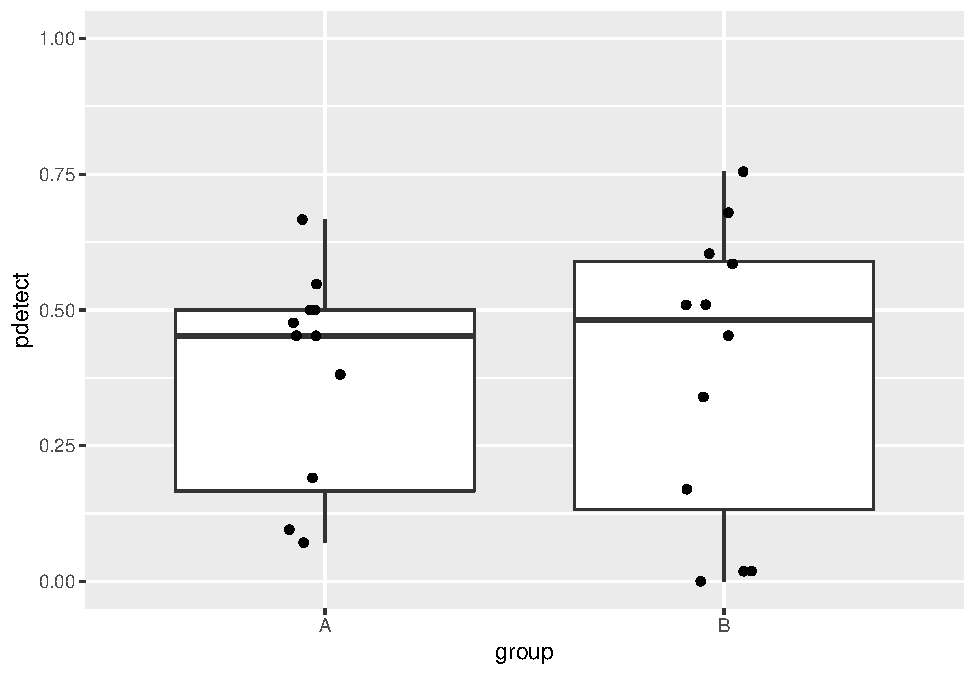
\includegraphics{survey_files/figure-latex/unnamed-chunk-2-1.pdf}

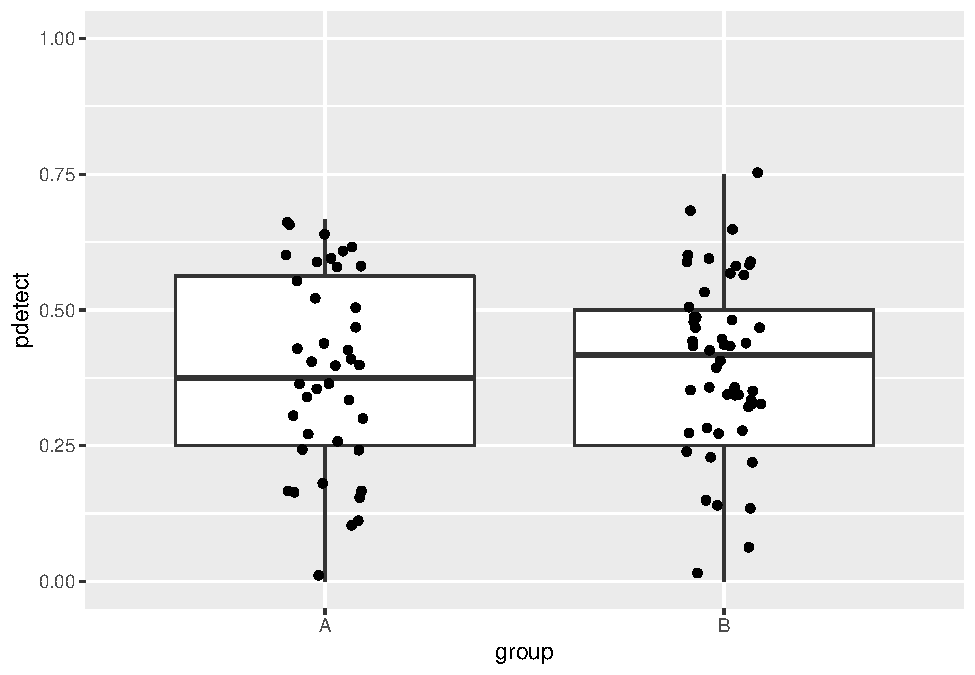
\includegraphics{survey_files/figure-latex/unnamed-chunk-4-1.pdf}

\begin{verbatim}
## # A tibble: 2 x 2
##   gender     n
##   <chr>  <int>
## 1 He        70
## 2 She       25
\end{verbatim}

\begin{verbatim}
## # A tibble: 6 x 2
##   age         n
##   <chr>   <int>
## 1 18 - 24    15
## 2 25 - 34    37
## 3 35 - 44    23
## 4 45 - 54    11
## 5 55+         6
## 6 NA          3
\end{verbatim}

\begin{verbatim}
## # A tibble: 3 x 2
##   education       n
##   <chr>       <int>
## 1 Bach           56
## 2 High School    25
## 3 Masters        14
\end{verbatim}

\begin{verbatim}
## # A tibble: 2 x 2
##   australia     n
##   <chr>     <int>
## 1 No           93
## 2 Yes           2
\end{verbatim}

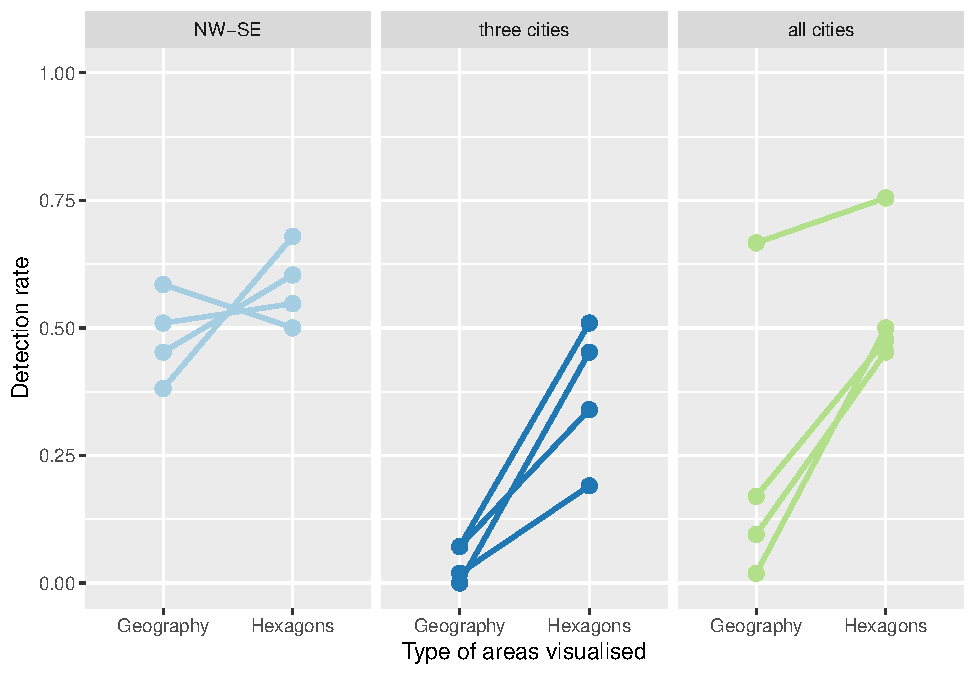
\includegraphics{survey_files/figure-latex/unnamed-chunk-7-1.pdf} 11 of
the 12 real distribution plots were found more often in the hexagon
display. This was better than expected. As even geographic distributions
were spotted in the hexagon lineup.

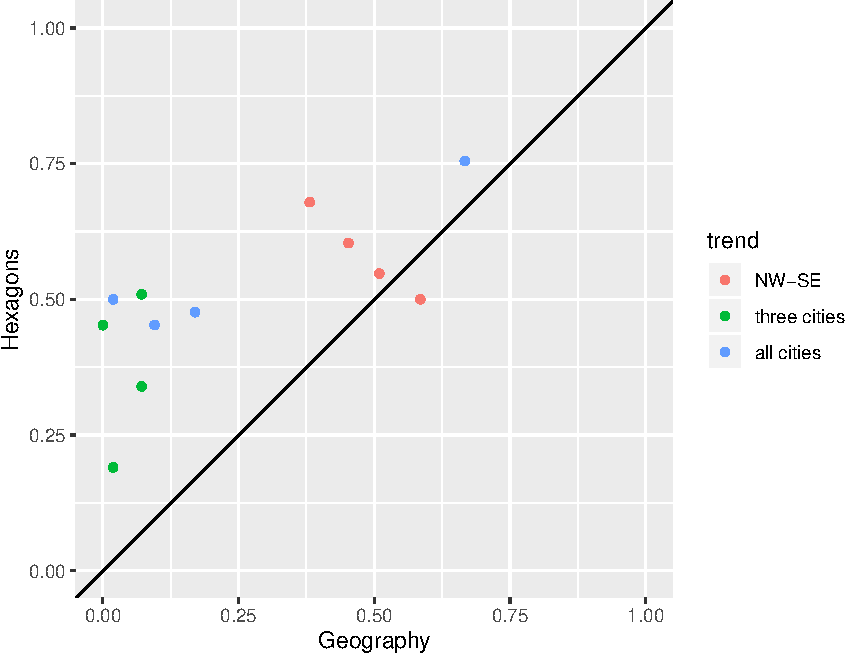
\includegraphics{survey_files/figure-latex/unnamed-chunk-8-1.pdf}

\begin{verbatim}
## [1] 0.004079185
\end{verbatim}

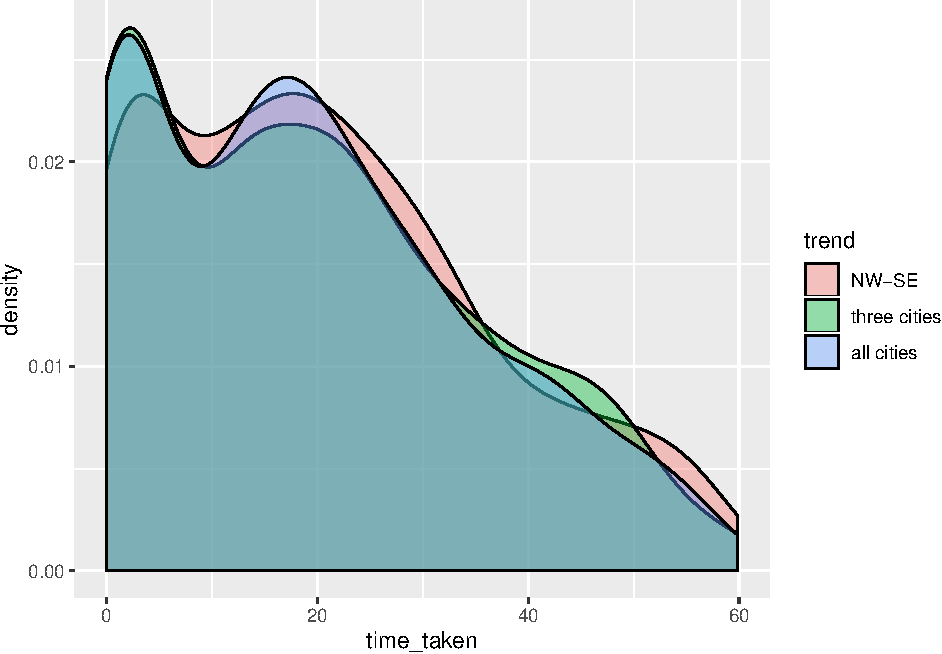
\includegraphics{survey_files/figure-latex/unnamed-chunk-9-1.pdf}
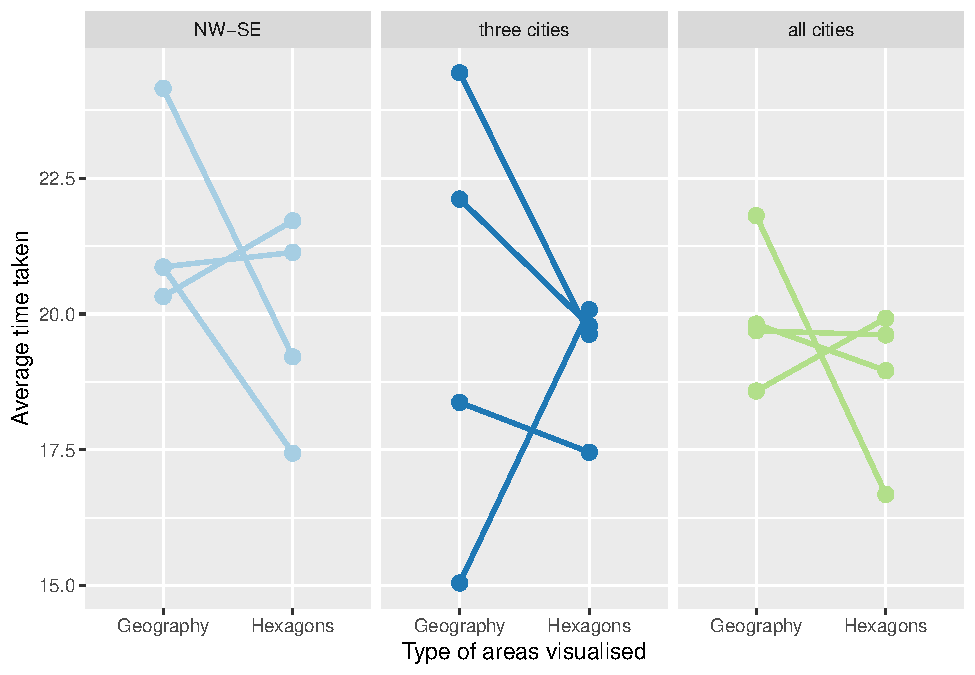
\includegraphics{survey_files/figure-latex/unnamed-chunk-9-2.pdf}

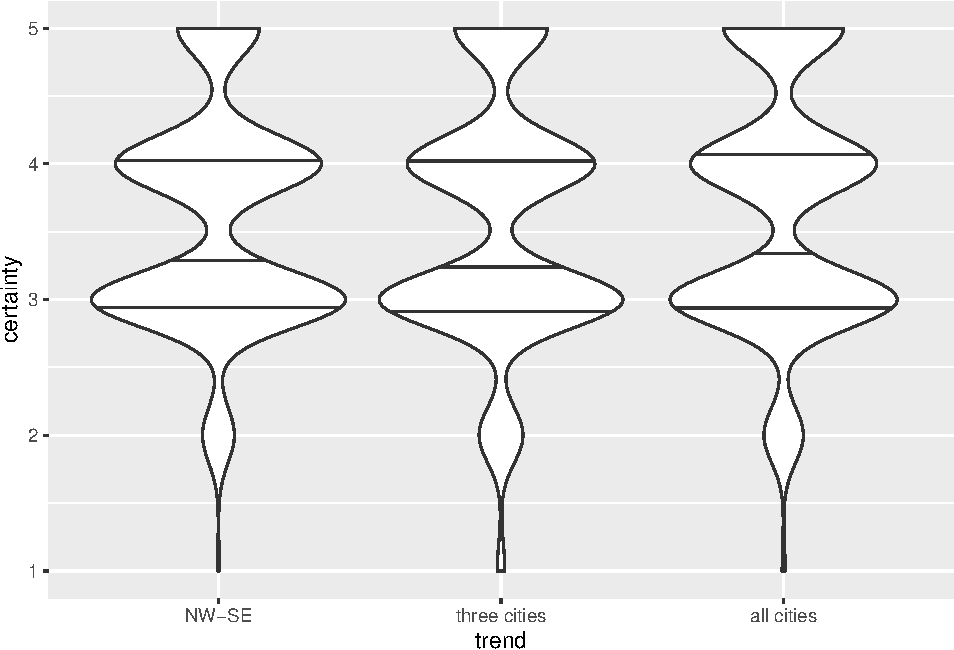
\includegraphics{survey_files/figure-latex/unnamed-chunk-10-1.pdf}
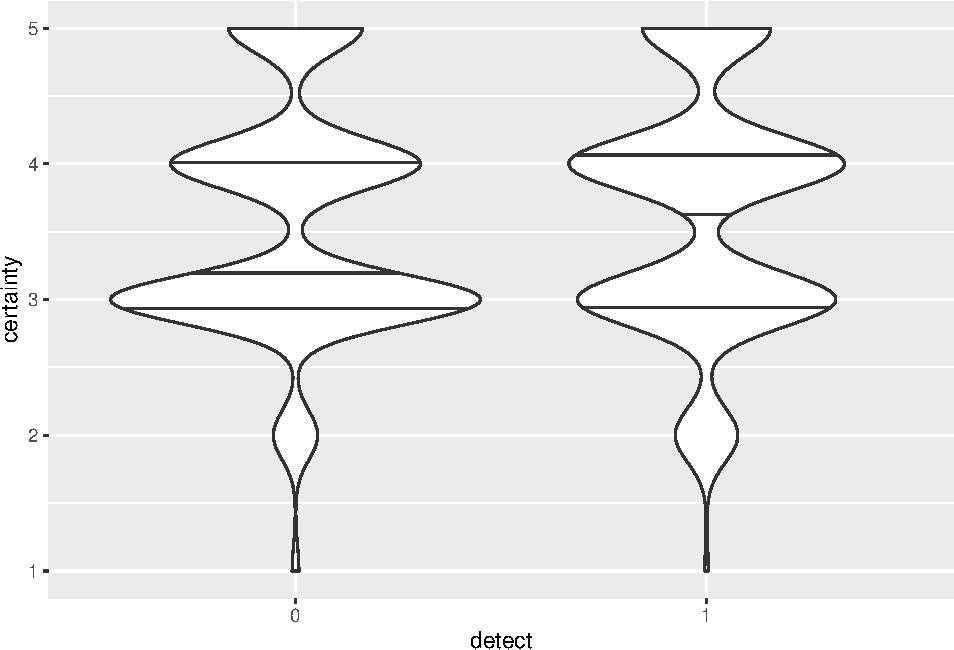
\includegraphics{survey_files/figure-latex/unnamed-chunk-10-2.pdf}

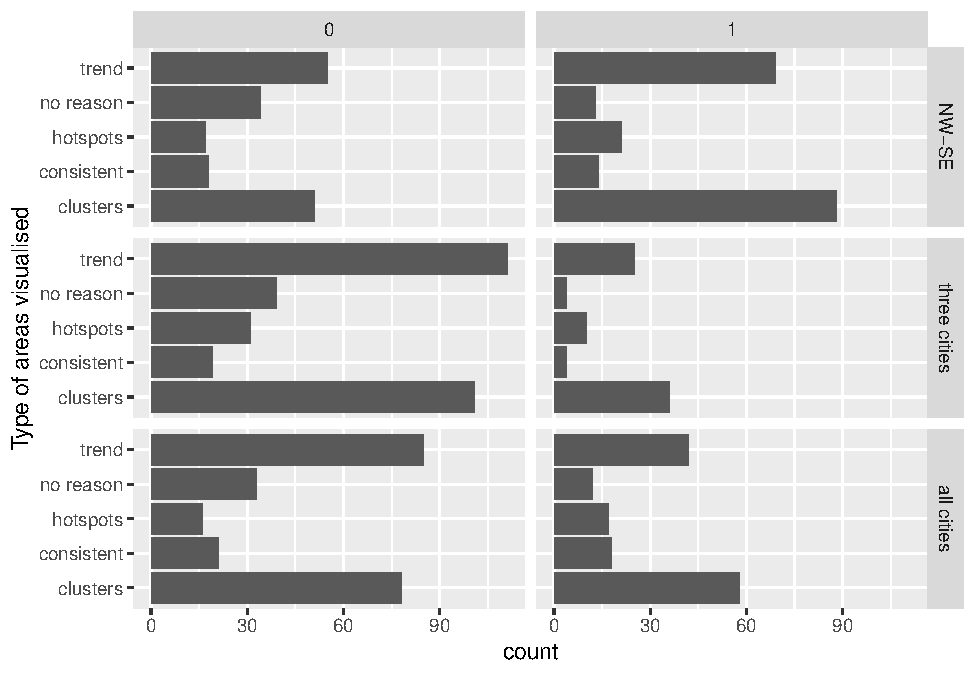
\includegraphics{survey_files/figure-latex/unnamed-chunk-11-1.pdf}

\hypertarget{probability-of-detection}{%
\subsection{Probability of detection:}\label{probability-of-detection}}

\hypertarget{time-taken}{%
\subsection{Time taken}\label{time-taken}}

\hypertarget{modeling-1}{%
\subsection{Modeling}\label{modeling-1}}

\hypertarget{discussion}{%
\section{Discussion}\label{discussion}}

\hypertarget{conclusion}{%
\section{Conclusion}\label{conclusion}}

The conclusion goes here.

\hypertarget{acknowledgment}{%
\section{Acknowledgment}\label{acknowledgment}}

The authors would like to thank\ldots{}

\hypertarget{bibliography-styles}{%
\section{Bibliography styles}\label{bibliography-styles}}

\newpage

\hypertarget{references}{%
\section{References}\label{references}}

\hypertarget{refs}{}
\leavevmode\hypertarget{ref-abs2016}{}%
``Australian Statistical Geography Standard (ASGS).'' 2018.
\emph{Australian Bureau of Statistics}. Australian Government.
\href{\%7Bhttps://www.abs.gov.au/websitedbs/D3310114.nsf/home/Australian\%20\%20\%20Statistical\%20Geography\%20Standard\%20(ASGS)\%7D}{\{https://www.abs.gov.au/websitedbs/D3310114.nsf/home/Australian   Statistical Geography Standard (ASGS)\}}.

\leavevmode\hypertarget{ref-sheets}{}%
Bryan, Jennifer, and Joanna Zhao. 2018. \emph{Googlesheets: Manage
Google Spreadsheets from R}.
\url{https://CRAN.R-project.org/package=googlesheets}.

\leavevmode\hypertarget{ref-SIEDAMD}{}%
Buja, Andreas, Dianne Cook, Heike Hofmann, Michael Lawrence, Eun-Kyung
Lee, Deborah F. Swayne, and Hadley Wlckham. 2009. ``Statistical
Inference for Exploratory Data Analysis and Model Diagnostics.''
\emph{Philosophical Transactions: Mathematical, Physical and Engineering
Sciences} 367 (1906): 4361--83.
\url{http://www.jstor.org/stable/40485732}.

\end{document}


